\chapter{\IfLanguageName{dutch}{Stand van zaken}{State of the art}}%
\label{ch:stand-van-zaken}

% Tip: Begin elk hoofdstuk met een paragraaf inleiding die beschrijft hoe
% dit hoofdstuk past binnen het geheel van de bachelorproef. Geef in het
% bijzonder aan wat de link is met het vorige en volgende hoofdstuk.

% Pas na deze inleidende paragraaf komt de eerste sectiehoofding.

\subsubsection{Inleiding}

In dit hoofdstuk worden een aantal zaken besproken met het oog op de contextualisering van de studie. Allereerst zal kort er in gegaan worden op de programmeertaal COBOL. Daarna wordt het verschil belicht tussen native en cross-platform ontwikkeling, elk met zijn eigen voor- en nadelen. Nadien volgt een bespreking van het .NET MAUI framework. Tenslotte zal ook het onderwerp real time toepassingen worden toegelicht.

\section{COBOL}
\subsection{Een korte geschiedenis van COBOL}
In de jaren vijftig was de informatica vooral gericht op de rekenkracht van computers, die vooral in de wiskunde en de wetenschap kon worden gebruikt. Financiële instellingen zagen echter ook de voordelen van computertoepassingen in het bedrijfsleven. In 1959 pleitte Mary Haws voor de ontwikkeling van een programmeertaal die kon worden gebruikt voor zakelijke doeleinden, zoals salarisadministratie, inventarisatie en analyse van bedrijfsgegevens \autocite{NMAH2013}.
In mei 1959 werd het Committee on Data Systems Languages, bekend als CODASYL, opgericht en gefinancierd door het Ministerie van Defensie om een nieuwe programmeertaal te ontwerpen en te ontwikkelen die voldeed aan de criteria van Mary Haws. Deze taal kreeg de naam COmmon Business-Oriented Language, of COBOL \autocite{Abby2023}.
De ontwikkeling van COBOL was gebaseerd op drie pijlers: leesbaarheid (de code moet leesbaar zijn voor zowel programmeurs als leken), overdraagbaarheid (toepassingen moeten snel en gemakkelijk kunnen worden overgezet naar een ander systeem) en flexibiliteit (de taal moet modulair genoeg zijn om zich aan te passen aan veranderende behoeften en technologieën) \autocite{Abby2023}.
In december 1960 slaagden zij erin COBOL te draaien op zowel een UNIVAC II systeem als een RCA machine \autocite{NMAH2013}.

\subsection{De huidige staat van COBOL}
Vandaag de dag wordt COBOL nog steeds gebruikt. De studie van \textcite{Reuters2017} toont aan dat 43 procent van de bankindustrie nog steeds steunt op COBOL. Sterker nog 95 procent van de pinautomaten steunen nog steeds aan op de programmeertaal. Volgens de studie van \textcite{MicroFocus2022} staan er momenteel 800 miljard lijnen COBOL in productie. Daarnaast gaven de bevraagden ook aan dat de hoeveelheid COBOL in productie nog zou verhogen. 
Voor 92 procent van de bevraagden blijven de COBOL-applicaties een strategische asset, die met der tijd ook gemoderniseerd zullen worden. Een voorbeeld hiervan is het integreren van cloud omgevingen en COBOL-applicaties \autocite{MicroFocus2022}.

\section{Native VS cross-platform development}
\subsection{Wat is native development?}
Van native ontwikkeling is sprake wanneer een programmeur een toepassing ontwikkelt die alleen op een bepaald platform kan draaien, zoals iOS of Android. Hiervoor moet de programmeur de programmeertaal en tools \autocite{Marchuk} gebruiken die het gekozen platform biedt.
Om native Android-toepassingen te schrijven, moet de ontwikkelaar Java of Kotlin gebruiken. Talen die native door het iOS-platform worden ondersteund zijn Objective-C en Swift \autocite{Schmitt2022}.

\subsection{Wat is cross-platform development}
Cross-platform ontwikkeling, ook bekend als multi-platform ontwikkeling, is een manier van ontwikkelen waarbij met één programmeertaal, en dus één codebase, een applicatie kan worden ontwikkeld die op verschillende platforms kan draaien \autocite{KotlinFoundation2022}.

\subsection{Een vergelijking tussen native en cross-platform development}
\begin{table}[H]
    \centering
    \begin{tabular}{|p{3.0in}|p{3.0in}|}
        \hline
            Voordelen & Nadelen 
            \\
        \hline
        \hline
        Hoge performantie
        
        De programmeertaal en API's van het doelplatform zijn geoptimaliseerd voor maximale prestaties.
            &
        Hogere ontwikkelkost
        
        Als een applicatie voor zowel iOS als Android moet worden ontwikkeld, moeten er twee verschillende teams van ontwikkelaars aan werken.
        \\\hline
        Uniforme UX (User eXperience)
        
        Elke native applicatie gebruikt dezelfde interface-elementen die door het platform worden geleverd. Hierdoor zien apps er consistenter uit en gedragen ze zich consistenter. Dit maakt een nieuwe applicatie intuïtiever en sneller te gebruiken.
            &
        Grotere ontwikkelteams
        
        Zoals gezegd zijn er meerdere teams nodig om verschillende applicaties voor de verschillende platforms te ontwikkelen. Binnen deze teams zal een groot aantal experts nodig zijn om hun expertise in te brengen tijdens het ontwikkelingsproces.
        \\\hline
        Toegang tot de gehele featureset van een platform
        
        Zoals vermeld in het eerste voordeel, kan native ontwikkeling gebruik maken van de API's die het platform biedt. Dit kan het gebruik zijn van de camera, GPS, pushmeldingen etc.
            &
        Verschillende codebases met risico op meer bugs
        
        Aangezien een applicatie meerdere programmeertalen vereist, is het gevolg dat er verschillende codebases zullen zijn.
        Dit kan leiden tot meer bugs omdat er meer regels code nodig zijn.
        \\\hline
        
            &
        Native applicaties kunnen verschillende logica-implementaties hebben
        
        Omdat elk platform een andere native programmeertaal biedt, kan het implementeren van bepaalde logica tot fouten leiden omdat de taal de logica anders interpreteert.
        Hetzelfde artikel kan bijvoorbeeld een verschillende prijs hebben op de twee platforms omdat de prijsberekening anders is geïmplementeerd.
        \\\hline
    \end{tabular}
    \caption{De voor- en nadelen van native development}
    \label{tab:nativeDevelopmentTable}
\end{table}

\begin{table}[H]
    \centering
    \begin{tabular}{|p{3.0in}|p{3.0in}|}
        \hline
        Voordelen & Nadelen 
        \\
        \hline
        \hline
        Deelbare code
        
        Met cross-platform ontwikkeling kunnen ontwikkelaars meerdere platforms bereiken met één enkele codebasis. Dit maakt een stuk code ook overdraagbaar van het ene project naar het andere.
            &
        Lagere performantie
        
        Omdat de cross-platform taal meerdere platformen moet kunnen aanspreken, kan de taal niet volledig worden geoptimaliseerd voor een bepaald platform, waardoor de prestaties op één platform iets langzamer zijn.
        \\\hline
        Sneller ontwikkelproces
        
        Er hoeven minder regels code te worden geschreven en getest, wat het ontwikkelingsproces aanzienlijk versnelt.
            &
        Beperkte toegang tot de gehele featureset van een platform
        
        Sommige platformen geven de moedertaal alleen toegang tot bepaalde API's of functies.
        Een voorbeeld hiervan is het weigeren van toegang tot pushmeldingen.
        \\\hline
        Hoge kosteneffectiviteit
        
        Kleinere ontwikkelingsteams kunnen meerdere platforms met dezelfde programmeertaal aanspreken, waardoor de ontwikkelingskosten dalen.
        &
        Beperkte UX-consistentie
        
        Cross-platform programmeertalen bieden elk hun eigen interfacecomponenten. Dit betekent dat cross-platform toepassingen vaak verschillende UI's hebben.
        \\\hline
        Gedeelde logica
        
        Het feit dat de toepassing is ontwikkeld met een enkele codebase betekent dat kan worden aangenomen dat de geïmplementeerde logica consistent is voor alle platforms.
        
        &
        
        \\\hline
    \end{tabular}
    \caption{De voor- en nadelen van cross-platform development}
    \label{tab:crossPlatformDevelopmentTable}
\end{table}

Zoals uit Tabel 2.1 \textcite{KotlinFoundation2023} en Tabel 2.2 \textcite{KotlinFoundation2023} op te maken is, is het debat over native VS cross-platform ontwikkeling niet eenvoudig. Elk heeft zijn voor- en nadelen, en voor elk project moet een grondige analyse worden gemaakt om te bepalen welke van deze zaken het belangrijkst zijn voor het project. Als een project hoge prestaties vereist en hoge ontwikkelingskosten minder belangrijk zijn, kunt u ervoor kiezen de toepassingen in de native programmeertaal te ontwikkelen.

Als het project daarentegen door een klein team wordt ontwikkeld en de applicatie zo snel mogelijk op beide platforms beschikbaar moet zijn, kan voor cross-platform ontwikkeling worden gekozen.

\section{.NET MAUI}
\subsection{Overzicht van wat .NET MAUI is en het doel ervan}
.NET MAUI staat voor .NET Multi-platform App UI en is de opvolger van Xamarin.Forms. Terwijl Xamarin.Forms diende als cross-platform programmeertaal die alleen op mobiele platformen kon worden gebruikt, kan .NET MAUI ook worden gebruikt om desktop en Smart TV applicaties te ontwikkelen. NET MAUI is vanaf de grond opgebouwd met uitbreidbaarheid en prestaties in het achterhoofd. Xamarin en .NET MAUI hebben veel overeenkomsten, maar de laatste maakt het ook mogelijk om platform-specifieke code toe te voegen \autocite{BradyGaster2020}.

\subsection{De werking van .NET MAUI}
\begin{figure}
    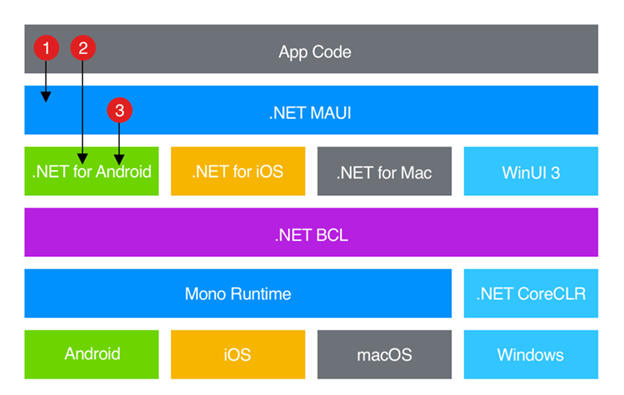
\includegraphics{maui_how_it_works}
    \centering
    \caption{Schematische voorstelling van de bouwstenen van .NET MAUI}
    \label{fig:mauiCompilationScheme}
\end{figure}
.NET MAUI voorziet in een framework per platform waarmee in C\# geschreven code kan worden gecompileerd voor het gewenste platform. Momenteel heeft .NET MAUI vier platformspecifieke frameworks: .NET voor Android, .NET voor iOS, .NET voor Mac en de Windows UI 3 bibliotheek. Elk van deze frameworks gebruikt de .NET Base Class Library, kortweg BCL, die fungeert als abstractie tussen de geschreven broncode en de verschillende platformen. De BCL vertrouwt op de .NET runtime om de toepassing te compileren. Ook hier zijn verschillende platformspecifieke tools voorzien. Zo is er de Mono runtime voor Android, iOS en macOS, en de .NET CoreCLR voor Windows desktop applicaties \autocite{Britch2023}.

Met BCL kunt u een toepassing maken die op verschillende platforms draait met dezelfde codebasis. Elk platform heeft echter zijn eigen manier om de gebruikersinterface te definiëren, evenals de manier waarop de verschillende elementen met elkaar communiceren en interageren. Dit is waar .NET MAUI u de keuze geeft om verschillende gebruikersinterfaces voor verschillende platformen te creëren of, omgekeerd, één gebruikersinterface voor alle platformen te creëren \autocite{Britch2023}.

\subsection{Een vergelijking tussen .NET MAUI en Xamarin}
Aangezien .NET MAUI de opvolger is van Xamarin.Forms, zijn er veel overeenkomsten, maar ook veel verschillen. In deze sectie worden de twee frameworks met elkaar vergeleken.

Het eerste grote verschil tussen .NET MAUI en Xamarin is de projectstructuur. In Xamarin wordt bij het aanmaken van een project een projectmap per platform aangemaakt, met als gevolg dat platformspecifieke code en resources (zoals fonts, afbeeldingen...) per project moeten worden onderhouden. Met de .NET MAUI wordt een projectmap aangemaakt die meerdere platformmappen bevat. In deze mappen wordt platformspecifieke code opgeslagen \autocite{Koleva2023}.

Het volgende verschil tussen de twee programmeertalen is de build tooling, .NET MAUI kan de cross-platform .NET CLI (Command Line Interface) gebruiken om projecten te compileren en uit te voeren. Terwijl Xamarin.Forms het .NET framework moet gebruiken om applicaties te bouwen \autocite{Kathiresan2022}.

Een derde belangrijk verschil tussen Xamarin.Forms en de .NET MAUI zijn de platform-specifieke API's. Xamarin biedt een enkele cross-platform API die werkt op Android, iOS en Windows. Met .NET MAUI wordt voor elk platform een API geleverd, waardoor ontwikkelaars kunnen profiteren van de functies van elk platform \autocite{UXDivers}.

Ten slotte kunt u met .NET MAUI kiezen om de GUI (Graphical User Interface) te bouwen met HTML (HyperText Markup Language) of XAML (Extensible Application Markup Language). Terwijl je met Xamarin.Forms alleen met XAML kon werken \autocite{Kathiresan2022}.

\subsection{Een blik op de toekomst van .NET MAUI}
\begin{figure}[H]
    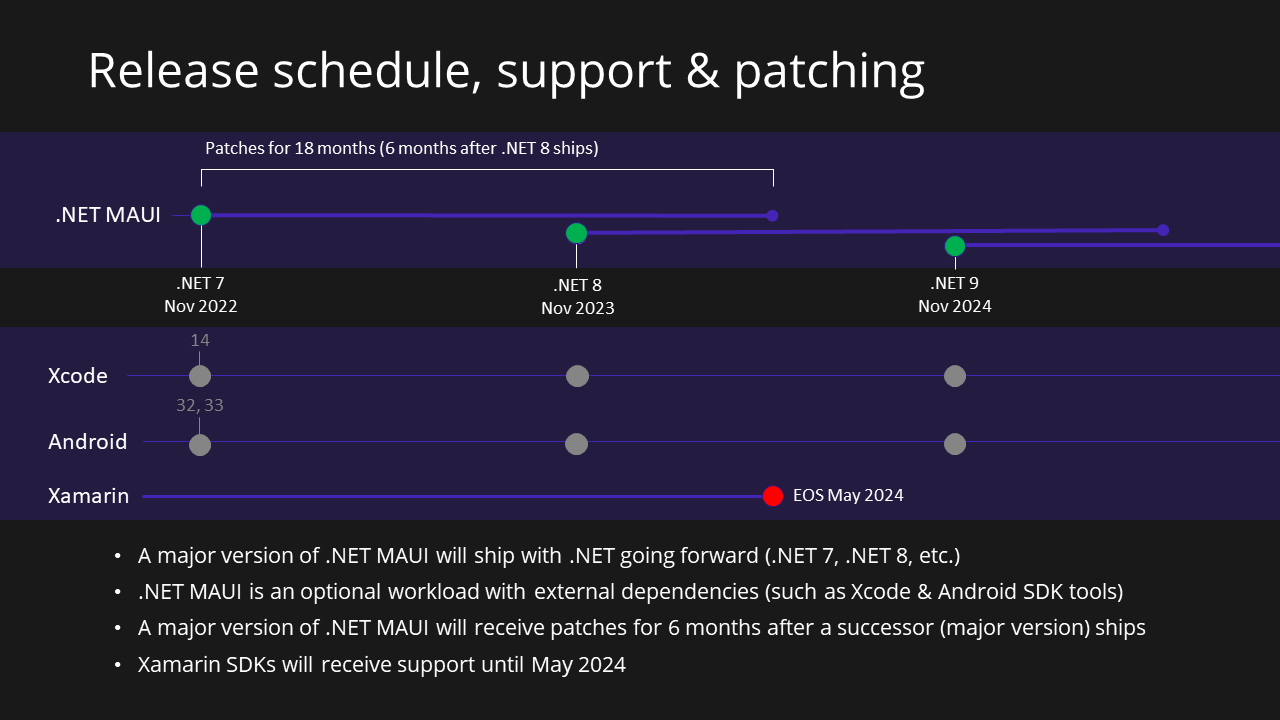
\includegraphics[scale=0.50]{maui_roadmap}
    \centering
    \caption{.NET MAUI release schema}
    \label{fig:mauiRoadMap}
\end{figure}

Elke nieuwe versie van .NET zal vanaf nu ook een major versie van .NET MAUI bevatten. Elk van deze major versies zullen 18 maanden ondersteuning krijgen \autocite{Ramel2022}.

Daarnaast zal de support voor Xamarin.Forms stopgezet worden in mei 2024. Concreet wil dit zeggen dat er geen updates of patches meer zullen uitgebracht worden voor Xamarin.Forms \autocite{Ramel2022}.

\section{Real-time applicaties}
\subsection{Definitie van een real-time applicatie}
Real-time computing verwijst naar computersystemen die zijn ontworpen om gegevensinvoer in real time te verwerken en erop te reageren, doorgaans binnen milliseconden of microseconden nadat gebeurtenissen zich hebben voorgedaan. 

De reactietijden moeten onmiddellijk aanvoelen en het systeem moet zonder vertraging of onderbreking doorgaan. 

Real-time computing is van cruciaal belang voor toepassingen die onmiddellijke en nauwkeurige gegevensverwerking vereisen, zoals industriële controle, medische toepassingen, luchtvaart, defensie, multimedia, games en financiële handelssystemen. 

Real-time computing vereist gespecialiseerde hardware- en softwarecomponenten, waaronder real-time besturingssystemen, real-time netwerken en synchrone programmeertalen, om het systeem binnen het gewenste tijdsbestek te laten functioneren.

\subsection{HyperText Transfer Protocol}
HTTP is het protocol dat ten grondslag ligt aan het internet. Het protocol wordt gebruikt om gegevensbronnen (zoals HTML, XML, JSON-documenten) op te vragen bij een server \autocite{Cloudflare}.

\begin{figure}[H]
    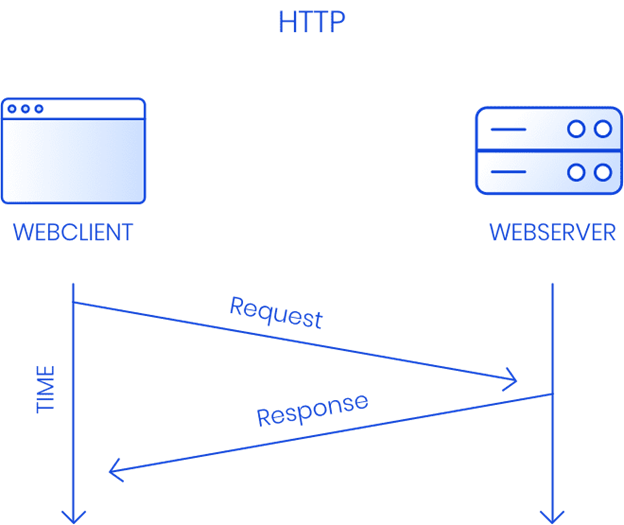
\includegraphics{client_server_scheme}
    \centering
    \caption{Schematische voorstelling van het server-client model}
    \label{fig:clientServerScheme}
\end{figure}

HTTP is een client-serverprotocol, wat betekent dat verzoeken om gegevens altijd door de client (ook bekend als de ontvanger) worden geïnitieerd. Het verzoek wordt naar de server gestuurd, die op zijn beurt het gevraagde document samenstelt en terugstuurt als antwoord op het verzoek \autocite{MDN2023}

\begin{figure}[H]
    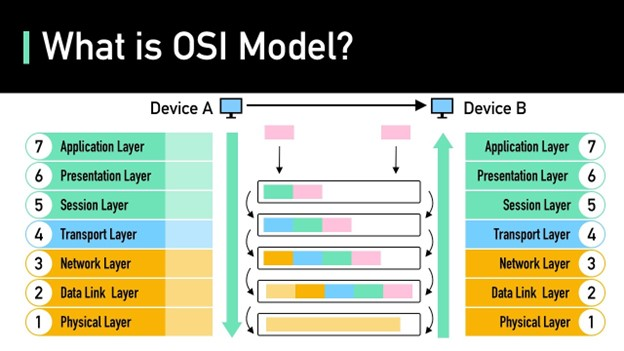
\includegraphics{osi_model}
    \centering
    \caption{Het OSI model}
    \label{fig:osiModel}
\end{figure}

Dit protocol werd oorspronkelijk voorgesteld door Tim Berners-Lee in 1989 en werd gebouwd bovenop de TCP- en IP-protocollen \autocite{MDN2023a}.

Het HTTP-protocol bevindt zich in de zevende laag (ook toepassingslaag genoemd) van het OSI-model \autocite{MDN2023}

De filosofie van HTTP rust op vier pijlers:\\

\begin{itemize}
    \item Uitbreidbaarheid

    De invoering van HTTP-headers in HTTP versie 1 (HTTP/1) \autocite{MDN2023a} maakt het mogelijk extra informatie toe te voegen aan verzoeken en antwoorden, zolang client en server deze overeenkomst aanvaarden \autocite{Paessler}.
    
    \item Staatloos
    
    Staatloos betekent dat tijdens en na het verzenden en ontvangen van een verzoek en antwoord geen informatie door de server wordt bijgehouden. Met andere woorden, elk verzoek dat de server ontvangt wordt onafhankelijk gezien en uitgevoerd. Een stateless protocol is ontworpen met het oog op schaalbaarheid. Afhankelijk van de werklast kunnen dus meerdere servers worden opgezet met dezelfde informatie, en elke server in de configuratie kan het verzoek ontvangen en verwerken \autocite{Paessler}.
    
    Om een toestand bij te houden kunnen HTTP-cookies worden gebruikt. Dit is mogelijk dankzij de bovengenoemde uitbreidbaarheid en maakt het mogelijk bepaalde informatie (zoals authenticatietokens) te delen tussen meerdere verzoeken \autocite{MDN2023}.
    
    \item Verbindingsloos
    
    Het HTTP-protocol wordt om twee redenen als verbindingsloos beschouwd. Omdat verbindingen worden gemaakt door de transportlaag (laag 4 van het OSI-model), valt het niet onder de verantwoordelijkheid van een applicatie laag (laag 7 van het OSI-model) applicatie \autocite{MDN2023}.
    
    Bovendien worden voor elk verzoek verbindingen gelegd tussen de client en de server. Zodra het verzoek is verwerkt, sluit de server de verbinding \autocite{Paessler}.
    
    \item Media onafhankelijk
    
    Zolang de client en de server weten hoe zij bepaalde door het MIME-type (Multipurpose Internet Mail Extensions) gespecificeerde gegevens moeten verwerken, kunnen de gegevens via het HTTP-protocol worden getransporteerd \autocite{Paessler}.
\end{itemize}

\subsubsection{De evolutie van het HTTP-protocol}
\emph{HTTP/0.9}

Aanvankelijk had het HTTP-protocol geen versienummer (aangegeven door het cijfer achter het teken /). Om de verschillende versies van elkaar te scheiden, kreeg de allereerste implementatie van het HTTP-protocol echter versienummer 0.9 \autocite{MDN2023a}.

Met verzoeken die bestonden uit een enkele regel bestaande uit het type verzoek en de naam van de gegevensbron, was deze versie van HTTP vrij primitief. Ook kon met deze versie alleen een GET-verzoek worden gedaan. Bijgevolg konden alleen gegevens worden gelezen \autocite{Grigorik}


\emph{HTTP/1.0}
HTTP-versie 1.0 werd uitgebracht in 1990, vijf jaar nadat versie 0.9 was geïntroduceerd, en voegde nieuwe functies toe om eerdere tekortkomingen te verhelpen:

\begin{itemize}
    \item HTTP-header
    
    Zoals hierboven vermeld, bestond een verzoek van versie 0.9 alleen uit de methode en de naam van de gegevensbron die werd opgevraagd \autocite{FulberGarcia2022}.
    Door de toevoeging van de HTTP-header kunnen nu metadata worden opgenomen in verzoeken en antwoorden, wat deze versie van het protocol flexibel en uitbreidbaar maakt \autocite{MDN2023a}.
    
    \item Versiebeheer
    
    Elk HTTP-verzoek bevat nu de gebruikte HTTP-versie \autocite{MDN2023a}.
    
    \item Statuscode
    
    Aan elk antwoord wordt een statuscode toegevoegd. Dit is een manier voor de cliënt om bij elk antwoord te controleren of het verzoek al dan niet correct is verwerkt \autocite{FulberGarcia2022}.
    
    \item Content-type
    
    Zoals hierboven vermeld, kunnen met de HTTP-header extra metadata aan een verzoek worden toegevoegd. Voor HTTP/1.0 is nu een inhoudstype in de header opgenomen, waardoor ook andere documenten dan HTML kunnen worden verzonden \autocite{FulberGarcia2022}.
    
    \item Extra methoden
    
    HTTP/1.0 heeft ten slotte twee nieuwe methoden toegevoegd, POST en HEAD. Dit zorgt ervoor dat gegevens nu zowel geschreven als gelezen kunnen worden \autocite{FulberGarcia2022}.
\end{itemize}


\emph{HTTP/1.1}
\begin{figure}
    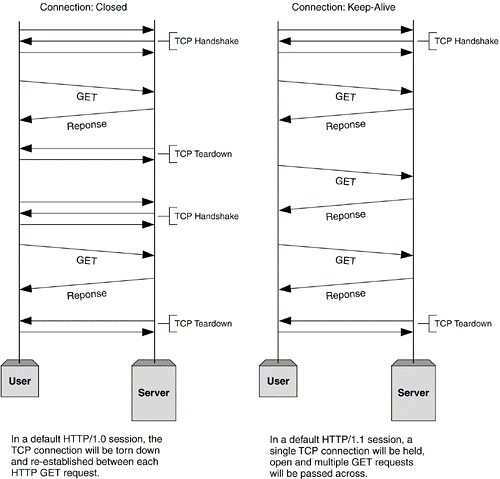
\includegraphics{http_1.0_vs_http_1.1_connections}
    \centering
    \caption{Schematische voorstelling van het verschil tussen niet-herbruikbare en herbruikbare connecties van respectievelijk HTTP/1.0 en HTTP/1.1}
    \label{fig:httpConnectionScheme}
\end{figure}

HTTP/1.1 werd een jaar na de release van HTTP/1.0 geïmplementeerd. Dit was slechts bedoeld als een verbetering van de 1.0-versie:

\begin{itemize}
    \item Host header
    
    Met HTTP/1.1 moest de client het host veld toevoegen aan de header van elke aanvraag. Vóór deze versie was dit niet verplicht. Dankzij dit veld kunnen verzoeken via een proxyserver naar de juiste server worden geleid, met andere woorden, als er verschillende domeinen naar dezelfde locatie verwijzen, kan er toch een onderscheid worden gemaakt om ervoor te zorgen dat het verzoek niet naar de verkeerde server gaat \autocite{FulberGarcia2022}.
    
    \item Persistente verbinding
    
    Zoals hierboven vermeld, moest de client in HTTP-versie 1.0 een verbinding maken voor elk verzoek dat hij wilde verzenden. In versie 1.1 kan de verbinding open worden gehouden totdat de client aangeeft dat hij de verbinding wil sluiten \autocite{MDN2023a}).
    
    \item Continue-status
    
    Vóór de invoering van de continue status konden sommige verzoeken niet door de server worden verwerkt. Als dit het geval was, werd het verzoek gewoon onbeantwoord afgewezen. Vanaf versie 1.1 kan een cliënt eerst de HTTP-headers van het verzoek aan de server doorgeven. Als de server antwoordt met de status continue (statuscode 100), weet de cliënt dat hij het hele verzoek kan doorsturen en een antwoord van de server kan verwachten \autocite{FulberGarcia2022}.
    
    \item Aanvullende methoden
    
    Versie 1.1 introduceert ook een aantal nieuwe methoden. Deze omvatten PUT, PATCH, DELETE, CONNECT, TRACE en OPTIONS \autocite{FulberGarcia2022}.
\end{itemize}


\emph{HTTP/2.0}

HTTP/2.0 werd uitgebracht in 2015, 18 jaar na 1.1. Het is echter nog niet op grote schaal ingevoerd. Het gebruik van HTTP/2.0 is dan ook een bewuste keuze van de ontwikkelaars \autocite{Ab}.
HTTP/2.0 brengt echter een aantal geweldige nieuwe functies die nieuwe mogelijkheden bieden, namelijk:

\begin{itemize}
    \item Multiplexing
    
    In versie 1.1 van het HTTP-protocol werden verzoeken om gegevens sequentieel verwerkt. Dat wil zeggen, het eerste HTML-document werd opgevraagd en geladen, dan het tweede document, ... tot alles geladen was. Dit kon echter tot problemen leiden als een bepaalde bron niet kon worden geladen omdat de rest van de bron werd opgehouden. Met HTTP/2.0 kan een enkele TCP-verbinding worden gebruikt om meerdere verzoeken om gegevens tegelijk te doen. Dit zorgt ervoor dat wanneer het bovengenoemde probleem zich voordoet, de resterende gegevens al kunnen worden geladen \autocite{Cloudflare}.
    
    \item Server push
    
    Vóór de invoering van HTTP/2.0 kon de server alleen gegevens naar de client pushen nadat deze een verzoek had verzonden. In versie 2.0 is echter server push geïmplementeerd. Hierdoor kan de server gegevens naar de client sturen nog voordat de client een verzoek naar hem heeft gestuurd. Dit lost prestatieproblemen met lange polling op \autocite{Grigorik2016}.
    
    \item Compressie van headers
    
    De toevoeging van HTTP-headers aan een verzoek vergroot de omvang van het verzoek. Dit kan leiden tot het langzamer laden van gegevens en het langzamer verwerken van gegevens door de client. Deze verzoeken kunnen kleiner worden gemaakt en sneller worden verwerkt door de headers te comprimeren. HTTP/1.1 deed dit al, maar versie 2.0 heeft een veel verfijnder compressie-algoritme, het HPACK-algoritme. Dit algoritme verwijdert alle overbodige informatie, waardoor verzoeken kleiner worden \autocite{Cloudflare}.
\end{itemize}

\subsection {WebSocket protocol}

Het WebSocket protocol is een relatief nieuw protocol. Het protocol werd voor het eerst beschreven in 2008 door Micahel Carter en Ian Hickson en kreeg algemene ondersteuning rond 2010 \autocite{Ably2020}.

In december 2011 publiceerde het IETF (Internet Engineering Task Force) de whitepaper die het WebSocket protocol beschreef onder de titel ``RFC 6455 - The WebSocket Protocol'' \autocite{Fette2011}.

Volgens de paper van \textcite{Fette2011} werd het WebSocket protocol ontwikkeld om real-time applicaties mogelijk te maken zonder het zogenaamde ``HTTP long polling'' te misbruiken.

Bij HTTP long polling stuurt de client een aanvraag uit naar de server. In plaats van direct te antwoorden en daarna de connectie te sluiten, wacht de server met antwoorden totdat er nieuwe data beschikbaar is. Na het uitsturen van het antwoord krijgt de server direct een nieuwe aanvraag van de client \autocite{Singh}. 

Het WebSocket protocol is full-duplex en laat bidirectionele communicatie toe. Concreet betekent dit dat in plaats van een aanvraag te sturen die enkel beantwoord wordt wanneer er nieuwe data is, is het nu mogelijk om data door te sturen naar de client zonder dat deze een aanvraag verstuurd heeft. Dit zorgt voor een betere performantie ten opzichte van het HTTP long polling \autocite{Fette2011}

\begin{figure}[H]
    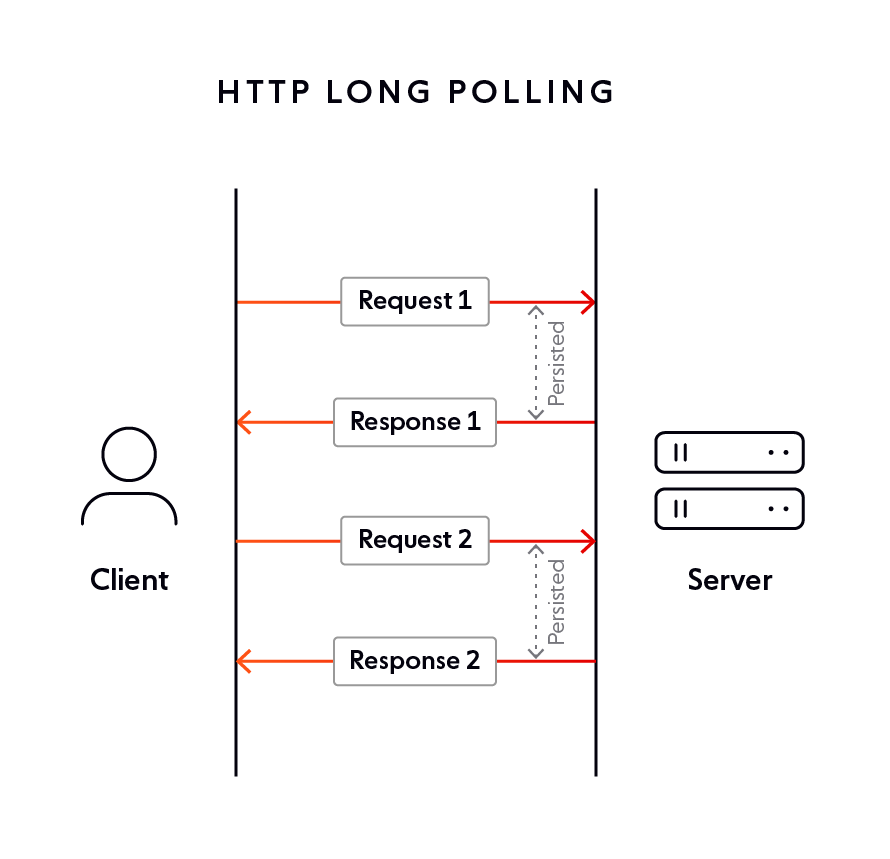
\includegraphics{http_long_polling}
    \centering
    \caption{Schematische voorstelling van HTTP long polling}
    \label{fig:httpLongPolling}
\end{figure}

\subsection{Real-time programmeren binnen het .NET ecosysteem}
De ASP.NET SignalR bibliotheek is beschikbaar voor real-time applicatieontwikkeling binnen het .NET ecosysteem. Deze bibliotheek maakt het mogelijk een tweerichtingscommunicatie op te zetten tussen een client en een server. De client kan met name bepaalde functies op de server aanroepen, maar de server kan ook functies opvragen bij de client \autocite{BradyGaster2020}.

In het traditionele client-server model kan alleen de client functies op de server aanroepen. Dit betekent dat als de gegevens zo actueel mogelijk moeten zijn, er extra logica moet worden geïmplementeerd om de server na een bepaald aantal seconden te polsen naar de (mogelijk) gewijzigde gegevens (deze implementatie wordt ook wel "long polling" genoemd). Dit kan leiden tot slecht presterende toepassingen \autocite{BradyGaster2020}.

Dankzij het gebruik van SignalR is het nu ook mogelijk dat de server functies gaat aanroepen op de client. Dit zorgt ervoor dat het hierboven getoonde voorbeeld op een veel performantere manier kan worden geïmplementeerd. Wanneer gegevens op de server worden gewijzigd, kan de server alle luisterende clients opdragen de nieuwe gegevens op te halen. Dit zorgt ervoor dat gegevens alleen worden opgevraagd wanneer de gegevens veranderen, in plaats van telkens na een bepaalde periode \autocite{BradyGaster2020}.